\section{Fazit}

\subsection{Heap oder List}

Die \textit{Holdback Queue} mit internem Heap und mit interner Liste wurden in den obigen Plots in verschiedenen Szenarien getestet und verglichen. In Abbildung \ref{fig:auf_heapList} ist zu erkennen, dass bei aufsteigender Eingabeliste kein Unterschied zwischen den beiden Implementierungen zu erkennen ist. Wie in Kapitel \ref{Problemstellungen} beschrieben, werden die Elemente bei der Liste jeweils hinten angefügt, während beim Heap alle Elemente an den nächsten leeren freien Index angefügt werden. Beim Anfügen an die Liste wird durch die Liste iteriert wodurch einen Komplexität von O(n) entsteht. Im Heap wird vom Wurzelelement aus das letzte freie Blatt gesucht und eine Komplexität von O(log(n)) entsteht. Für das Entfernen eines Elements, wird das erste Element der Liste abgeschnitten und mit dem Rest der Liste weitergearbeitet was eine Komplexität von O(1) zur Folge hat. Beim Heap hingegen muss das Wurzelelement entfernt und dann das neue Wurzelelement bestimmt werden was in O(2*log(n)) resultiert. Die Gesamtkomplexität ist folglich O(n) für die Liste und O(3*log(n)) für den Heap. Der Heap sollte also schneller sein als die Liste.\\
Nun wurde im Benchmark allerdings immer die \textit{Delivery Queue} mit eingebunden. Es lässt sich schließen, dass diese so ineffizient ist, dass die Optimierungen der \textit{Holdback Queue} wenig Einfluss auf den Gesamtprozess hat. Egal wie schnell ein Teilprozess Elemente verarbeitet, wenn der Nachfolgeprozess nicht mindestens genauso schnell ist, bildet sich im Nachfolgeprozess ein Stau und die Optimierung des ersten Teilprozesses wird hinfällig. Zur Bestätigung dieser Vermutung wurde eine Messung mit den einzelnen \textit{Holdback Queues} durchgeführt (siehe Abbildung \ref{fig:real_hbqOnly}). Gemessen wurde hierbei nur der Prozess vom Eintritt der Nachrichten in die \textit{Holdback Queue}, bis zum Verlassen mit realer Eingabeliste.

\begin{figure}[htbp]
\begin{center}
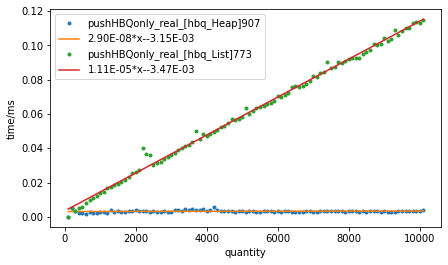
\includegraphics[scale=0.65]{Latex/Bilder/Plots/real_hbqOnly.png}
\caption{\label{fig:real_hbqOnly} real - vgl. List, Heap ohne Delivery Queue} 
\end{center}
\end{figure}

Hier ist der Unterschied zwischen den Implementierungen mit interner Liste und internem Heap klar zu erkennen. Die Steigung der Trendlinie der \textit{Holdback Queue} mit interner Liste ist um ca. 30° steiler. \\ Die Umsetzung der \textit{Holdback Queue} mit einem internen Heap um die Elemente besser zu sortieren erweist sich also als effizienter. Bei einer neuen Implementierung dieser gesamten Aufgabe sollte also auch die \textit{Delivery Queue} und nicht nur die \textit{Holdback Queue} optimiert werden. Eine mögliche Herangehensweise hierfür wäre, die Sortierung der \textit{Delivery Queue} zu verändern, sie also zum Beispiel absteigend zu sortieren. Dafür müsste analysiert werden, ob wirklich genauso viele Elemente in die Queue eingefügt, wie auch wieder gelöscht werden, wie es in Kapitel \ref{dlq} angenommen wurde. Ein Ausgang dieser Analyse wird vermutlich sein, dass nach Terminierung der \textit{Holdback Queue} keine weiteren Elemente mehr in die \textit{Delivery Queue} eingefügt werden müssen. Somit werden auch keine mehr aus dieser gelöscht. Somit wäre also eine \textit{Delivery Queue} mit absteigender Liste effizienter, da das von Erlang angebotene 'aneinander-pipen' von Elementen schneller ist, als der '++' Operator.

\subsection{Limit der Delivery Queue}

Die Plots aus Abbildung \ref{fig:real_heapListPercent} und Abbildung \ref{fig:rand_heapListPercent} zeigen, wie groß der Einfluss des \textit{Delivery Queue} Limits auf die Gesamtlaufzeit ist. Je kleiner dieses Limit hier ist, desto schneller ist der Prozess. Da die Elemente ab Erreichen einer \textit{Holdback Queue} Größe von 2/3-tel des \textit{Delivery Queue} Limits von der \textit{Holdback} an die \textit{Delivery Queue} weitergegeben werden, wird bei einem kleineren \textit{Delivery Queue} Limit mit kleineren \textit{Holdback Queues} gearbeitet. Ein Element in eine kleinere Liste oder einen kleineren Heap einzufügen, benötigt dementsprechend weniger Zeit, da weniger Iterationen durchgeführt, beziehungsweise Teilbäume gesucht werden müssen. Allerdings vergrößert sich hierdurch das Risiko, dass Elemente verloren gehen, weil der \textit{Delivery Queue} Speicher nicht groß genug ist. Wenn Elemente zu schnell eingefügt werden, dann werden die ältesten Nachrichten bereits gelöscht, bevor die \textit{Clients} diese lesen konnten. Das \textit{Delivery Queue} Limit sollte also an die Lesegeschwindigkeit der \textit{Clients} angepasst werden.

\subsection{Pattern Matching}
\textit{Pattern Matching}, um die Effizienz der \textit{Holdback Queue} zu erhöhen, hat sich anhand der Plots aus Abbildung \ref{fig:auf_hbq_pattern} und Abbildung \ref{fig:real_hbqAll}, im Widerspruch zur Annahme aus Kapitel \ref{erwartungen}, eher als wenig maßgebend erwiesen. 

Vorherige Auswertungen der Plots haben bereits gezeigt, dass die \textit{Delivery Queue} einen starken Einfluss auf die Laufzeiten hat. Dementsprechend wurde eine weitere Messung durchgeführt (siehe Abbildung \ref{fig:auf_hbqOnly_pattern}). In dieser wird mit einer Eingabeliste, welche bis zu 25000 Elementen in aufsteigend sortierter Reihenfolge hat, noch einmal die \textit{Holdback Queue} mit und ohne \textit{Pattern Matching} gemessen. Die Queue ohne \textit{Pattern Matching} ist anfangs noch leicht ineffizienter, dessen Trendlinie verläuft aber leicht flacher als die der \textit{Holdback Queue} mit \textit{Pattern Matching}. Da die Zeiten der Messdurchläufe hier sehr gering sind ist die Streuung sehr hoch. Diese ist aber sehr willkürlich und wird somit nicht weiter ausgewertet.

\begin{figure}[htbp]
\begin{center}
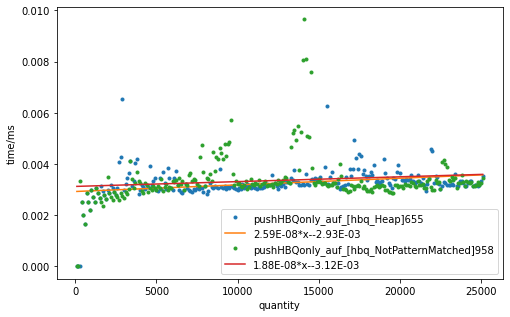
\includegraphics[scale=0.6]{Latex/Bilder/Plots/auf_heapOnly_pattern.png}
\caption{\label{fig:auf_hbqOnly_pattern} auf - vgl. Heap ohne Delivery Queue (mit und ohne PatternMatching)} 
\end{center}
\end{figure}

\newpage 
Zum Vergleich der beiden verschiedenen Implementierungen folgt ein Codeauszug aus der \textit{Holdback Queue} ohne \textit{Pattern Matching}. Dieses Beispiel soll die Tiefe des Codes und nicht die Funktionalität veranschaulichen, daher wird die Initialisierung mancher Parameter nicht gezeigt. \\

\begin{lstlisting}
loop(HBQ, DLQ, Datei, Pos, DLQLimit) ->
	receive
		{From, {request, pushHBQ, [NNr, Msg, TSclientout]}} ->
			if 
				NNr < ExpNr ->
				true ->
					if
						Pos < (DLQLimit*2/3) ->
						true -> 
							if
								SNNr == ExpNr ->
								    ...
								true ->									
									...
					        end
			        end
	        end;
\end{lstlisting}

Das nächste Beispiel zeigt einen Auszug der \textit{Holdback Queue} mit \textit{Pattern Matching}. Auch hier wurden wieder große Teile des Codes entfernt, um nur die Tiefe zu verdeutlichen. Statt fast die gesamte Funktion in einem Block zu implementieren, werden hier die zwei Hilfsfunktionen \textit{pushHBQ/8} und \textit{pushHBQHelp/10} verwendet. 
\newpage
\begin{lstlisting}
loop(HBQ, DLQ, Datei, Pos, DLQLimit) ->
	receive
		{From, {request, pushHBQ, [NNr, Msg, TSclientout]}} ->
			pushHBQ([NNr, Msg, TSclientout, erlang:timestamp()], ExpNr, HBQ, DLQ, Datei, Pos, DLQLimit, From);
    ...
    
% --------------------------------------------------------------------------%
pushHBQ([NNr, _Msg, _TSclientout, _TShbqin], ExpNr, HBQ, DLQ, Datei, Pos, DLQLimit, From) when NNr < ExpNr -> ...;
pushHBQ([NNr, Msg, TSclientout, TShbqin], _ExpNr, HBQ, DLQ, Datei, Pos, DLQLimit, From) when Pos < (DLQLimit*2/3) -> ...;
pushHBQ([NNr, Msg, TSclientout, TShbqin], ExpNr, HBQ, DLQ, Datei, Pos, DLQLimit, From) ->
	pushHBQHelp([NNr, Msg, TSclientout, TShbqin], ExpNr, DLQ, Datei, Pos, DLQLimit, DLQMsg, SNNr, TempHBQ, From).

pushHBQHelp([NNr, Msg, TSclientout, TShbqin], ExpNr, DLQ, Datei, Pos, DLQLimit, DLQMsg, SNNr, TempHBQ, From) when SNNr == ExpNr -> ...;
pushHBQHelp([NNr, Msg, TSclientout, TShbqin], ExpNr, DLQ, Datei, Pos, DLQLimit, DLQMsg, SNNr, TempHBQ, From) -> ...;
\end{lstlisting}

Auffällig ist, dass die erste Variante trotz der vielen Ebenen übersichtlicher wirkt als die zweite. Durch die vielen Parameter (\textit{pushHBQHelp/10} hat entsprechend zehn Parameter), welche den Hilfsfunktionen im unteren Auszug übergeben werden, strecken sich die Funktionsköpfe und sind schwer zu lesen. Letztendlich ist der Code aber kompakter und beim Hinzufügen weiterer Ebenen wird die Variante mit dem \textit{Pattern Matching} wieder übersichtlicher.\\
Die Zeitmessungen haben erwiesen, dass keine Variante effizienter als die andere ist. 
Laut dem von Erlang gegebenen \textit{'Efficiency Guide'} \footnote{\url{https://www.erlang.org/doc/efficiency_guide/functions.html#pattern-matching}} wird das \textit{Pattern Matching} vom Kompiler zu einem \textit{switch-case} generiert. 

\begin{lstlisting}
% Pattern Matching
foo(X, []) -> X;
foo(X, [Head|Tail]) -> Tail.
% wird zu Code kompiliert, welcher folgendem Beispiel gleicht:
foo(X,Y) ->
    case Y of
        [] -> X;
        [Head|Tail] -> Tail
    end.
\end{lstlisting}

\newpage
Das \textit{switch-case} Statement im Allgemeinen ist sehr effizient. Der Kompiler erstellt eine Tabelle mit den möglichen Werten, welche alle den gleichen Typen wie die übergebene Variable haben. Statt dann wie beim \textit{if-else} Statement jede Bedingung zu prüfen, kann beim Aufruf des \textit{switch-case} Statements der richtige Wert aus der Tabelle gesucht und der zugehörige Pfad ausgewählt werden. Ab fünf Fällen wird der \textit{switch-case} deutlich effizienter als der \textit{if-else}. Die Tabellen werden nun intern als \textit{Lookup-Table} oder \textit{Hash-List} implementiert und somit können alle Elemente innerhalb der gleichen Zeit gefunden werden (frei nach \cite{geeksforgeeks}). Da in dem Code dieser Aufgabe nie mehr als fünf Fälle geprüft werden, ist das Optimieren durch \textit{Pattern Matching} hier nicht ausschlaggebend. Außerdem benötigen die Hilfsfunktionen und die vielen Parameter mehr Speicher und Zeit, diesen zu schreiben und zu lesen. Die kompilierte \textit{beam-Datei} der \textit{Holdback Queue} ohne \textit{Pattern Matching} ist 1kB (16\%) kleiner als die der anderen Queue. Im Plot der Abbildung \ref{fig:real_hbqAll} ist ab einer Eingabelistengröße von ca. 10000 auch zu erkennen, dass die \textit{Holdback Queue} ohne \textit{Pattern Matching} (die orange Trendlinie) leicht effizienter als die mit ist. \\
Allgemein gilt also, dass beim Verwenden von wenig Parametern und wenig Hilfsfunktionen \textit{Pattern Matching} die bessere Variante ist. Besonders, wenn mit vielen Fällen innerhalb der Funktion gearbeitet wird. In dieser Implementierung ist aber der Verzicht auf Hilfsfunktionen effizienter, da ansonsten zu viele Parameter übergeben werden müssen und auf Maschinenebene mehr Code gelesen wird. 

\subsection{Alternative Anwendung}

Die \textit{Holdback} und \textit{Delivery Queue} in dieser Form können in vielen anderen Anwendungsgebieten genutzt werden. Dabei sollten aber Modifizierungen hinsichtlich der Sortieralgorithmen innerhalb der \textit{Holdback Queue} vorgenommen werden. Wenn Werte aus einer großen Menge komplett zufällig an den \textit{Server} gesendet werden und mehrere \textit{Clienten} nun die Werte in richtiger Reihenfolge erwarten, dann sollte die Größe der \textit{Holdback Queue} fast so groß, wie die der Wertemenge sein, damit keine Werte durch einen \textit{Overflow} der \textit{Holdback Queue} verloren gehen. Die interne Struktur der \textit{Holdback Queue} wäre dann der Heap. Effizient wäre diese abstrakte Datenstruktur, da die Sortierung der Werte unabhängig von der Ausgabe an die \textit{Clients} stattfindet. Würde im Vergleich nur die \textit{Holdback Queue} genutzt werden und diese würde die Elemente über einen Heap sortieren, dann würde das kleinste Element als Wurzel solange dort stehen, bis alle \textit{Clients} es empfangen haben und erst danach könnte das neue kleinste Element gesucht werden.\\
Angenommen die Elemente werden in aufsteigender Reihefolge an den \textit{Server} geschickt, wäre nur eine \textit{Delivery Queue} am sinnvollsten. Die Größe muss nicht der Wertemenge entsprechen, sondern hängt von der Geschwindigkeit der \textit{Clients} ab.